%%%%%%%%%%%%%%%%%%%%%%%%%%%%%%%%%%%
% PART I: User's manual
%%%%%%%%%%%%%%%%%%%%%%%%%%%%%%%%%%%

\part{User's manual}
\chapter{A short \GLOBES\ tour}

To be written later: Short introduction such as ``With the following lines we obtain ...''
without detailed description of parameters. Should contain all most important functions of \GLOBES\ --
overview of main functions in \tabl{stdfunctions}.
Maybe: in form of long example which involves everything (for example: our famous bar plot, which involves
systematics, correlations, degeneracies and thus the full set of \GLOBES\ functions without being too
complicated in the application software part).

\begin{table}[t]
\begin{center}
\begin{tabular}{p{1.8cm}p{4.5cm}p{8.6cm}}
\hline
Function & Purpose & Parameters \ra\ Result \\
\hline
{\tt Chi} & $\chi^2$ with systematics only \newline (all initialized exps.) & ($\{ \theta_{12}, \theta_{13}, \theta_{23}, \deltacp , \sdm , \ldm, \hat{\rho_1},... , \hat{\rho_n} \}$)  \newline \ra\  $\chi^2$ \\[0.1cm]
{\tt SingleChi} & $\chi^2$ with systematics only \newline (only one experiment) & $(\{ \theta_{12}, \theta_{13}, \theta_{23}, \deltacp , \sdm , \ldm, \hat{\rho}_{N_{\mathrm{exp}}} \}, \, N_{\mathrm{exp}} )$   \newline \ra\ $\chi^2$ \\[0.1cm]
{\tt ChiTheta} & $\chi^2$ with systematics and correlations: Projection onto $\theta_{13}$-axis (all exps.) &  ($ \theta_{13}, \, \{ \theta_{12}, \theta_{23}, \deltacp , \sdm , \ldm, \hat{\rho_1}, ... , \hat{\rho_n} \}$) \newline \ra\  $\{ \chi^2, \theta_{12}, \theta_{23}, \deltacp , \sdm , \ldm, \hat{\rho_1}, ... , \hat{\rho_n} , N_{\mathrm{Iter}} \}$ \\[0.1cm]
{\tt Single-} \newline {\tt ChiTheta} & $\chi^2$ with systematics and correlations: Projection onto $\theta_{13}$-axis (one exp.) &  ($ \theta_{13}, \, \{ \theta_{12}, \theta_{23}, \deltacp , \sdm , \ldm,  \hat{\rho}_{N_{\mathrm{exp}}} \}, \, N_{\mathrm{exp}}$) \newline \ra\  $\{ \chi^2, \theta_{12}, \theta_{23}, \deltacp , \sdm , \ldm, \hat{\rho}_{N_{\mathrm{exp}}} , N_{\mathrm{Iter}} \}$ \\[0.1cm]
{\tt ChiDelta} & $\chi^2$ with systematics and correlations: Projection onto $\deltacp$-axis (all exps.) &  ($\deltacp, \, \{ \theta_{12}, \theta_{13}, \theta_{23},  \sdm , \ldm, \hat{\rho_1}, ... , \hat{\rho_n} \}$) \newline \ra\  $\{ \chi^2, \theta_{12}, \theta_{13}, \theta_{23}, \sdm , \ldm, \hat{\rho_1}, ... , \hat{\rho_n} , N_{\mathrm{Iter}} \}$ \\[0.1cm]
{\tt Single-} \newline {\tt ChiDelta} & $\chi^2$ with systematics and correlations: Projection onto $\deltacp$-axis (one exp.) &  ($ \deltacp, \, \{ \theta_{12}, \theta_{13}, \theta_{23}, \sdm , \ldm,  \hat{\rho}_{N_{\mathrm{exp}}}  \}, \, N_{\mathrm{exp}}$) \newline \ra\  $\{ \chi^2, \theta_{12}, \theta_{13}, \theta_{23},  \sdm , \ldm, \hat{\rho}_{N_{\mathrm{exp}}} , N_{\mathrm{Iter}} \}$ \\[0.1cm]
{\tt ChiTheta-} {\tt Delta} & $\chi^2$ with systematics and correlations: Projection onto $\deltacp$-$\theta_{13}$-plane (all exps.) &  ($\theta_{13}, \, \deltacp, \, \{ \theta_{12}, \theta_{23},  \sdm , \ldm,  \hat{\rho_1}, ... , \hat{\rho_n} \}$) \newline \ra\  $\{ \chi^2, \theta_{12}, \theta_{23}, \sdm , \ldm,  \hat{\rho_1}, ... , \hat{\rho_n} , N_{\mathrm{Iter}} \}$ \\[0.1cm]
{\tt SingleChi-} {\tt Theta- } {\tt Delta} & $\chi^2$ with systematics and correlations: Projection onto $\deltacp$-$\theta_{13}$-plane (one exp.) &  ($ \theta_{13}, \, \deltacp, \, \{ \theta_{12}, \theta_{23}, \sdm , \ldm,  \hat{\rho}_{N_{\mathrm{exp}}} \}, \, N_{\mathrm{exp}}$) \newline \ra\  $\{ \chi^2, \theta_{12},  \theta_{23},  \sdm , \ldm, \hat{\rho}_{N_{\mathrm{exp}}} , N_{\mathrm{Iter}} \}$ \\[0.1cm]
{\tt ChiNP} & $\chi^2$ with systematics and correlations: Projection onto $N$-parameter hyper-plane (one exp.) & ??? to be defined \\[0.1cm]
{\tt Single-} {\tt ChiNP} & $\chi^2$ with systematics and correlations: Projection onto $N$-parameter hyper-plane (one exp.) & ??? to be defined \\[0.1cm]
{\tt ChiAll} & Lokal minimum of $\chi^2$ with respect to all parameters (all exps.) &
($ \{ \theta_{13}, \theta_{12}, \theta_{23}, \deltacp , \sdm , \ldm,  \hat{\rho_1}, ... , \hat{\rho_n} \}$) \newline \ra\  $\{ \chi^2, \theta_{13}, \theta_{12}, \theta_{23},$ \newline \hspace*{1.4cm} $ \deltacp , \sdm , \ldm,  \hat{\rho_1}, ... , \hat{\rho_n} , N_{\mathrm{Iter}} \}$ 
\\[0.1cm]
{\tt Single-} {\tt ChiAll} & Lokal minimum of $\chi^2$ with respect to all parameters (one exp.) &  ($ \{ \theta_{13}, \theta_{12}, \theta_{23}, \deltacp , \sdm , \ldm,  \hat{\rho}_{N_{\mathrm{exp}}} \}, \, N_{\mathrm{exp}}$) \newline \ra\  $\{ \chi^2, \theta_{13}, \theta_{12}, \theta_{23}, \deltacp , \sdm , \ldm, \hat{\rho}_{N_{\mathrm{exp}}} , N_{\mathrm{Iter}} \}$ \\[0.1cm]
\hline
\end{tabular}
\end{center}
\caption{\label{tab:stdfunctions} The \GLOBES\ standard function to obtain a $\chi^2$-value for all or one of the initialized experiments. The curly brackets refer to the parameters to be transferred in form of a list. The parameter $\hat{\rho}_i \equiv \rho_i/\bar{\rho}_i$ refers to the matter density scaling factor, which is $1.0$ for leaving the matter density profile unchanged. Note that all functions but {\tt Chi} and {\tt SingleChi} are using minimizers which have to be initialized with {\tt SetInputErrors} and {\tt SetStartingValues} first.}
\end{table}

\chapter{Getting started with \GLOBES }

In this first chapter of the user's manual, we assume that the \GLOBES\ software is readily installed on your computer system. We demonstrate how to load pre-defined experiments and re-obtain information about them. However, we only secondarily discuss the usage of \GLOBES\ in your specific programming language, such as C, Mathematica, or others. Thus, you should be familiar of how to load \GLOBES\ on your computer system before reading this chapter. An example of how to use \GLOBES\ with C can be found on page~\pageref{ex:c}. 

\example{Using \GLOBES\ with C}{\label{ex:c}

Here comes some complete C-code with a very simple example of how to use \GLOBES .
 
}

\begin{table}[t]
\begin{center}
\begin{tabular}{lll}
\hline
Quantities & Examples & Units \\
\hline
Angles & $\theta_{13}$, $\theta_{12}$, $\theta_{23}$, $\deltacp$ & Radians  \\
Mass squared differences & $\sdm$, $\ldm$ & $\mathrm{eV}^2$ \\
Matter densitities & $\rho_i$ & $\mathrm{g}/\mathrm{cm}^3$ \\
Baseline lengths & $L_i$ & $\mathrm{km}$ \\
Energies & $E_\nu$ & $\mathrm{GeV}$ \\  
Fiducial masses & $m_{\mathrm{Det}}$ & $\mathrm{kt}$ \\
Time intervals & $t_{\mathrm{run}}$ & $\mathrm{yr}$ \\
Source powers & $P_{\mathrm{Source}}$ & ??? \\
% Integrated luminosities & $m_{\mathrm{Det}} \, t_{\mathrm{run}}$ & $\mathrm{kt \cdot yr}$ \\
Cross sections & $\sigma_{\mathrm{CC}}$ &  ???? \\
\hline
\end{tabular}
\mycaption{\label{tab:units} Quantities used in \GLOBES , examples of these quantities, and their standard units in the application software.}
\end{center}
\end{table}

Throughout the programming interface of \GLOBES , the software needs to transfer parameters to and from the software core. Unless the Experiment Definition Module \EDM , the programming interface only uses one set of units for each type of quantity in order to avoid confusion about the definition of individual parameters. \tabl{units} summarizes the units of the most important quantities used in \GLOBES .

\begin{table}[t]
\begin{center}
\begin{tabular}{llp{7cm}c}
\hline
Experiment & Filename & Short description & Refs. \\
\hline 
\multicolumn{3}{l}{\underline{Conventional beams:}} \\
??? & & \\[0.1cm]

\multicolumn{3}{l}{\underline{First-generation superbeams:}} \\
\JHFSK\ ($\nu$) & {\tt JHFSK.exp} & JHF (J-PARC) to Super-Kamiokande, neutrino running &  \cite{Huber:2002mx,Huber:2002rs} \\
\JHFSK\ ($\bar\nu$)& {\tt JHFSKanti.exp} & JHF (J-PARC) to Super-Kamiokande, antineutrino running &  \cite{Huber:2002rs} \\
\NUMI\  ($\nu$), OA $9 \, \mathrm{km}$ & {\tt NUMI9.exp} & NuMI with off-axis angle of $9 \, \mathrm{km}$ for $L=712 \, \mathrm{km}$, neutrino running & \cite{Huber:2002rs} \\
\NUMI\  ($\bar{\nu}$), OA $9 \, \mathrm{km}$ & {\tt NUMI9anti.exp} & NuMI with off-axis angle of $9 \, \mathrm{km}$ for $L=712 \, \mathrm{km}$, antineutrino running & \cite{Huber:2002rs} \\
\NUMI\  ($\nu$), OA $12 \, \mathrm{km}$ & {\tt NUMI12.exp} & NuMI with off-axis angle of $12 \, \mathrm{km}$ for $L=712 \, \mathrm{km}$, neutrino running & \cite{Huber:2002rs} \\
\NUMI\  ($\bar{\nu}$), OA $12 \, \mathrm{km}$ & {\tt NUMI12anti.exp} & NuMI with off-axis angle of $12 \, \mathrm{km}$ for $L=712 \, \mathrm{km}$, antineutrino running & \cite{Huber:2002rs} \\
\SPL\  ($\nu$) & {\tt SPL.exp} & SPL (CERN), neutrino running &  ??? \\
\SPL\  ($\bar\nu$) & {\tt SPLanti.exp} & SPL (CERN), antineutrino running & ??? \\[0.1cm]
 
\multicolumn{3}{l}{\underline{Superbeam upgrades:}} \\
\JHFHK\ ($\nu$) & {\tt JHFHK.exp} & JHF (J-PARC) to Hyper-Kamiokande superbeam upgrade, neutrino running &  \cite{Huber:2002mx,Huber:2002rs} \\
\JHFHK\ ($\bar\nu$)& {\tt JHFHKanti.exp} & JHF (J-PARC) to Hyper-Kamiokande superbeam upgrade, antineutrino running &  \cite{Huber:2002mx,Huber:2002rs} \\[0.1cm]

\multicolumn{3}{l}{\underline{Neutrino factories:}} \\
\NuFactI\ & {\tt NuFact.exp} & Initial stage neutrino factory, symmetric operation in both polarities & \cite{Huber:2002mx} \\
\NuFactII\  & {\tt NuFact2.exp} & Advanced stage neutrino factory, symmetric operation in both polarities & \cite{Huber:2002mx,Huber:2003ak} \\[0.1cm]

\multicolumn{3}{l}{\underline{Reactor experiments:}} \\
\ReactorI\ & {\tt Reactor.exp} & Small reactor experiment with identical near and far detectors & \cite{Huber:2003pm} \\
\ReactorII\ & {\tt Reactor2.exp} & Large reactor experiment with identical near and far detectors & \cite{Huber:2003pm} \\[0.1cm]

\multicolumn{3}{l}{\underline{$\beta$-Beams:}} \\
\Beta\ ($\nu$) & {\tt BETA.exp} & $\beta$-Beam, neutrino running & ??? \\
\Beta\ ($\bar\nu$) & {\tt BETAanti.exp} & $\beta$-Beam, antineutrino running & ??? \\
\hline
\end{tabular}
\end{center}
\mycaption{\label{tab:experiments} Different pre-defined experiments, their filenames (to be used in {\tt LoadExperiment}), their short description, and the references in which they are defined. Note that all experiments use in their standard configurations one year of running time. Details about the experiment parameters can be obtained with {\tt InfoExperiment}(Experiment number) after they have been loaded.}
\end{table}

In principle, \GLOBES\ can handle any number of different long-baseline experiments simultaneously. This means that their $\chi^2$-values are added {\em after} the minimization over the independent systematics parameters and {\em before} any minimization over the oscillation parameters. Though the simplest case of only one experiment may be most often used, more experiments are useful in many cases. For example, running a superbeam some years in the neutrino mode and some years in the antineutrino mode can be, to a first approximation, simulated by the combination of two such experiments.\footnote{Note that in this case the systematics parameters are minimized over independently, which means that this approach does not allow correlations among the systematics parameters. Therefore, the neutrino factory with the symmetric operation of both polarities is encapsulated into a single experiment.} Another example is the test of synergetic effects among different experiment types. Thus, \GLOBES\ has an internal (initially empty) list of currently initialized experiments. To add a pre-defined experiment to this list, one can use the function {\tt LoadExperiment}:
\begin{function}
{\tt LoadExperiment}$($``filename'' $)$ adds a single experiment to the list of currently loaded experiments. All currently loaded experiments are evaluated simultaneously (if not explicitely stated otherwise), \ie , their $\chi^2$-values are added.
\end{function}
A list of pre-defined experiment types, their filenames, their short descriptions, and the references of their definitions can be found in \tabl{experiments}. To remove all experiments from the evaluation list, one uses {\tt ClearExp}:
\begin{function}
{\tt ClearExp}$()$ removes all experiments from the evaluation list.   
\end{function}
Both functions do not return anything. Thus, one can either add an experiment to the internal evaluation list, or remove all experiments from this list. After adding an experiment, it gets an internal experiment number $N_{\mathrm{exp}}$ assigned in the order of the addition, which is starting from zero and running to the number of experiments minus one. Therefore, one will be able to access the individual experiment by its number later.

Since the pre-defined experiments in \tabl{experiments} are given for one year running time, specific target masses, and specific source powers, it is useful to change these parameters of the individual experiments:
\begin{function}
{\tt SetRunningTime}$(N_{\mathrm{exp}},t_{\mathrm{run}})$ sets the running time of experiment number $N_{\mathrm{exp}}$ to $t_{\mathrm{run}}$ years.
\end{function}
 \begin{function}
{\tt SetTargetMass}$(N_{\mathrm{exp}},m_{\mathrm{Det}})$ sets the fiducial mass of experiment number $N_{\mathrm{exp}}$ to $m_{\mathrm{Det}}$ kilotons.
\end{function}
\begin{function}
{\tt SetSourcePower}$(N_{\mathrm{exp}},P_{\mathrm{Source}})$ sets the source power of experiment number $N_{\mathrm{exp}}$ to $P_{\mathrm{source}}$. The definition of the source power depends on the experiment type: ... (MISSING).
\end{function}
Thus, these functions also demonstrate how to use the assigned experiment number.

A useful function to re-obtain the information about the initialized experiments is the function {\tt InfoExperiment}:
\begin{function}
{\tt InfoExperiment}$()$ prints a list of the initialized functions with their experiment numbers and their most important parameters to the standard output.
\end{function} 
Especially, after changing individual parameters, such as baseline or target mass, this information can be useful to check the changes. Another useful function is {\tt ShowChannels}, which prints the initialized oscillation channels for a specified experiment:
\begin{function}
{\tt ShowChannels}$(N_{\mathrm{exp}})$ prints the information about the oscillation channels of the experiment with the number $N_{\mathrm{exp}}$ to the standard output.
\end{function}

Compared to an existing experiment, which uses real data, a future experiment uses simulated data. Thus, the {\em true parameter values} and their results in form of the reference rate vectors are simulated. After setting the true parameter values, the {\em fit parameter values} can be varied in order to obtain information on the measurement performance for the given set of true parameter values. Therefore, it is often useful to show the results of a future measurement as function of the true parameter values for which the reference rate vectors are computed -- at least within the currently allowed ranges. The true parameter values for the vacuum neutrino oscillation parameters have to be set by the functions {\tt SetVacuumParameters} and {\tt SetRates} {\em before} any evaluation function is used and {\em after} the experiments have been initialized and the experiment parameters have been adjusted which could change the rates (such as baseline or target mass). Any matter effects are then included automatically depending on the experiment definitions.
\begin{function}
{\tt SetVacuumParameters}$(\{\theta_{12}, \theta_{13}, \theta_{23}, \deltacp , \sdm , \ldm \})$ sets the neutrino oscillation parameters to be used to compute the reference rate vector in vacuum.
\end{function}
\begin{function}
{\tt SetRates}$( )$ computes the reference rate vector for the neutrino oscillation parameters set with {\tt SetVacuumParameters}. 
\end{function}
Finally, an initialization sequence for \GLOBES\ could look like this:
\begin{quote}
{\tt
ClearExp(); \\
InitExperiment("JHFHK.exp"); \\
SetRunningTime(0, 2.0); \\
InitExperiment("JHFHKanti.exp"); \\
SetRunningTime(1, 6.0);\\
MInfoExperiment(); \\
SetVacuumParameters(\{0.55, 0.16, 3.14/4, 3.14/2, 7e-5, 2e-3\}); \\
SetRates();
} 
\end{quote}
This piece of code initializes the JHF (J-PARC) to Hyper-Kamiokande superbeam upgrade with two years of neutrino running and six years of antineutrino running, \ie, an overall running time of eight years. The final configuration is then printed to the standard output and the reference rate vector is set to the chosen parameter values.

\chapter[Calculating $\chi^2$ with systematics only]{Calculating $\boldsymbol{\chi^2}$ with systematics only}

Calculating a $\chi^2$-value with or without systematics, but no correlations and degeneracies, is the simplest and fastest possibility to obtain high-level information on an experiment. I general, \GLOBES\ uses the six independent oscillation parameters $\theta_{12}$, $\theta_{13}$, $\theta_{23}$, $\deltacp$, $\sdm$, $\ldm$, as well as the matter density of each experiment. Thus, there are six plus the number of experiments parameters determining the rate vectors. Using the matter densities in addition to the oscillation parameters will allow the simulation of matter density uncertainties: In this approach, the matter densities can be treated as parameters to be measured by the experiments within certain limits, where the limits are given by the observed precision of the matter density profile. Defining a independent matter density for each experiment is necessary if the baselines are completely uncorrelated. For correlated or even identical baselines, one may rather want to encapsulate the experiments into a single experiment definition. 

\example{Correlation between $\stheta$ and $\deltacp$}{
\label{ex:corrth13dcp}

A typical application for {\tt Chi} and {\tt SingleChi} is the visualization of two-parameter correlations. For example, to show the correlation between $\stheta$ and $\deltacp$ at a large neutrino factory with four years of running time for each polarity, one can use the following code:
\begin{quote}
{\tt
/\% Experiment initialization: \%/ \\
ClearExp(); \\
 InitExperiment("{\tt NuFact2.exp}"); \\
 SetRunningTime(0,4.0); \\
 MInfoExperiment(); \\
\\
/\% Set reference rate vector: \%/ \\
th12=arcsin(sqrt(0.8))/2; sdm=7e-5; \\
th23=3.14/4; ldm=2e-3; \\
th13=arcsin(sqrt(0.001))/2; dcp=3.14/2; \\
\mbox{SetVacuumParameters(\{th12, \, th13, \, th23, \, dcp, \, sdm, \, ldm\}); }\\
 SetRates(); \\
\\
/\% Compute chi-square matrix: \%/ \\
for (float x=-4; x<-2; x=x+2/50) \\
\hspace*{0.5cm} for (float y=0; y<200; y=y+200/50) \{ \\
\hspace*{1cm} theth13 = arcsin(sqrt(10$\hat{\, \, \,}$x))/2; \\
\mbox{\hspace*{1cm} Print(\{x,y,Chi(\{th12, theth13,  th23,  y, sdm, ldm, 1.0\}) \}) \};}
}
\end{quote}

The resulting matrix can then be plotted as a contour plot (2 d.o.f.):
\begin{center}
\colorbox{white}{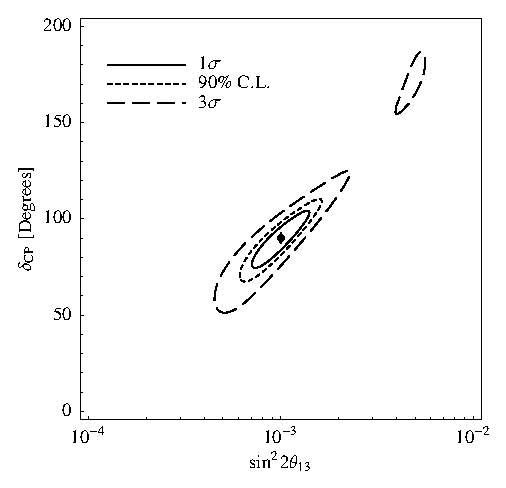
\includegraphics[width=8cm]{correx}}
\end{center}

}

Keeping all oscillation parameters and matter densities fixed, one can use the following functions to obtain the total $\chi^2$ of all specified oscillation channels including systematics:
\begin{function} 
{\tt Chi}$(\{ \theta_{12}, \theta_{13}, \theta_{23}, \deltacp , \sdm , \ldm, \hat{\rho_1}, \hdots , \hat{\rho_n} \})$  returns the total added $\chi^2$ of all loaded experiments.
\end{function}
\begin{function}
 {\tt SingleChi}$(\{ \theta_{12}, \theta_{13}, \theta_{23}, \deltacp , \sdm , \ldm, \hat{\rho}_{N_{\mathrm{exp}}} \}, \, N_{\mathrm{exp}} )$  returns the total $\chi^2$ of the experiment number $N_{\mathrm{exp}}$.
\end{function}
Note that the result of {\tt Chi} corresponds to the sum of all of the {\tt SingleChi}'s of the loaded experiment. This equality will not hold for the minimizors in the next sections anymore. In both functions, one has to give the matter density scaling factor $\hat{\rho_i}$ for each of the used experiments. The effect of this scaling factor depends on the type of the matter density profile, which is given in the  experiment definition. For a constant matter density, it is simply the ratio of the matter density and the average matter density specified in the experiment definition, \ie , $\hat{\rho_i} \equiv \rho_i/\bar{\rho}_i$. For a matter density profile, it is an overall scaling factor: The matter density in each layer is multiplied by this factor. In most cases one wants to take a scaling factor of $1.0$ here, which simply means taking the matter density profile as it is given in the experiment definition. Moreover, note that its effect is in general small for short baselines. An example of how to use  {\tt Chi} (or {\tt SingleChi}) can be found on page~\pageref{ex:corrth13dcp}.  

The treatment of systematics is done by the usage of auxiliary systematics parameters, which are taken completely uncorrelated among different oscillation channels, and treated with simple Gaussian statistics. One such example is the signal normalization error, \ie, an error to the overall normalization of the signal. For illustration, we assume that the signal event rate in the $i$th bin $s_i^0$ of one oscillation channel is altered by the overall normalization auxiliary parameter of this channel, \ie , 
\be
 s_i = s_i(n_s) = s_i^0 \cdot (1 + n_s),
\ee
where $n_s$ is the signal normalization parameter. The total number of events in the $i$th bin $x_i$ also includes the background event rates $b_i$, \ie, $x_i = s_i + b_i$, which may have their own systematics parameters.
In order to implement an overall signal normalization error $\sigma_{n_s}$,  the $\chi^2$, which includes all event rates $x_i$ of all bins, is minimized over the auxiliary parameter $n_s$:
\be
 \hat{\chi^2} = \underset{n_s}{\mathrm{min}} \left(  \chi^2(n_s, \hdots) + \frac{(n_s)^2}{\sigma_{n_s}^2} \right).
\ee 
This minimization is done independently for all auxiliary parameters of this oscillation channel. The total $\chi^2$ for the considered experiment is finally obtained by repreating this procedure for all oscillation channels and adding their $\chi^2$-values. In general, the situation is more complicated because of the usage of many systematical errors. More details about systematics parameters and the definition of signal, background, and oscillation channels can be found in the \EDM\ part of this book, too.

The systematics minimization of an experiment can be easily switched on and off, \ie, one can also compute the $\chi^2$ without even taking into account systematics:
\begin{function}
{\tt SetSystematics}$(N_{mathrm{exp}}, \, sys)$ switches the systematics minimization for experiment $N_{\mathrm{exp}}$ on (sys=1) or off (sys=0).
\end{function}
This function can be especially useful for the test of the impact of systematics.
??? Wie einzelne Systematik-Parameter ein und ausschalten? Sonst individuell nicht testbar! ??? Verweis auf appendix? 

\chapter[Calculating $\chi^2$-projections: how one can include correlations]{Calculating $\boldsymbol{\chi^2}$-projections: how one can include correlations}

This chapter deals with the rather complicated issue of $n$-parameter correlations. Since it has before this software  not been possible to include the full $n$-parameter correlations in the high-dimensional parameter space with reasonable effort, it is the core part of this software  -- as well as its strength. Of course, calculating $\chi^2$-projections is somewhat more complicated than using systematics only. Therefore, we use a simple step by step introduction to the problem. 

\section{Introduction}

In principle, the precision of an individual parameter measurement including correlations can be obtained as the projection of the $n$-dimensional fit manifold onto the respective axis. Similarly, one can project the fit manifold onto a plane, such as the $\stheta$-$\deltacp$-plane, if one wants to explicitely show this correlation with all the other parameter correlations included. In practice, this projection is very difficult: a grid-based method would need $(N_{\mathrm{grid}})^n$ function calls of {\tt Chi} or {\tt SingleChi} to calculate the precision including the full $n$-parameter correlation, where $N_{\mathrm{grid}}$ is the number of points in each direction of the lattice. For example, taking only $N_{\mathrm{grid}}=20$ and $n=7$ (six oscillation parameters and matter density) would mean more than one billion function calls of {\tt Chi} or {\tt SingleChi}. One can easily image that this is too much for any sophisticated application.

The solution to this problem is using a local $n$-dimensional minimizer instead of a grid-based method. It turns out that such a minimizer can include a full $6$-parameter correlation with of the order of $1\, 000$ function calls of {\tt Chi} or {\tt ChiNew}. It is a standard method which can be found in every good book for standard numerical calculation routines. Thus, for each point on the projection axis/plane, one can obtain a result within about $10$ to $30$ seconds on a modern computer, which means that the complete measurement precision for one fixed true parameter set can be obtained in as much as $10$ to $15$ minutes. One can easily imagine that such a minimizer makes more sophisticated applications possible with the help of overnight calculations, such as showing the dependencies on the true parameter values.

This approach also has a major disadvantage: One can not simply program a robust grid-based code and let it run, since using a local minimizer always means that one may end up in an unwanted local minimum and not in the investigated one. Thus, one has to use some (analytical or numerical) knowledge on the topology of the fit manifold and start the local minimizer close enough to the investigated solution. Fortunately, this can be done quite straightfoward in most cases, since the structure of the neutrino oscillation formulas does not cause very complicated topologies of the fit manifolds. Especially, the are plenty of analytical discussions of this issue, which means that one can implicitely use this knowledge to obtain better predictions for the measurement performances. Note that, since one can easily find the global fit minimum at the best-fit values, any solution found with the local minimizer makes the measurement performance worse. Thus, one can only run the danger to obtain a too optimistic solution if one does not find the other local minima below the chosen confidence level.

In many cases, the fit manifold is restricted by the knowledge from earlier experiments. For example, the knowledge on the solar parameters will in most cases be supplied by the solar neutrino experiments. If the external precision of a parameter is at the time of the measurement better than the one of the experiment itself, one has to impose some external knowledge on this parameter. This external knowledge may reduce the $n$-dimensional fit manifold in the respective direction. In the most extreme case, keeping all parameters but the measured one fixed in the analysis means that all parameters are determined externally with infinitively high precisions. Thus, using the projection method on the axis/plane of interest is a reasonable approach. The inclusion of external input in \GLOBES\ is done by the use of Gaussian {\em priors}: We assume that an external measurement has determined the measured parameter to be at the central value (called {\em starting value}) with a $1 \sigma$ Gaussian error (called {\em input error}). The explicit definition of these priors will be shown in the next section.

\begin{figure}[t]
\begin{center}
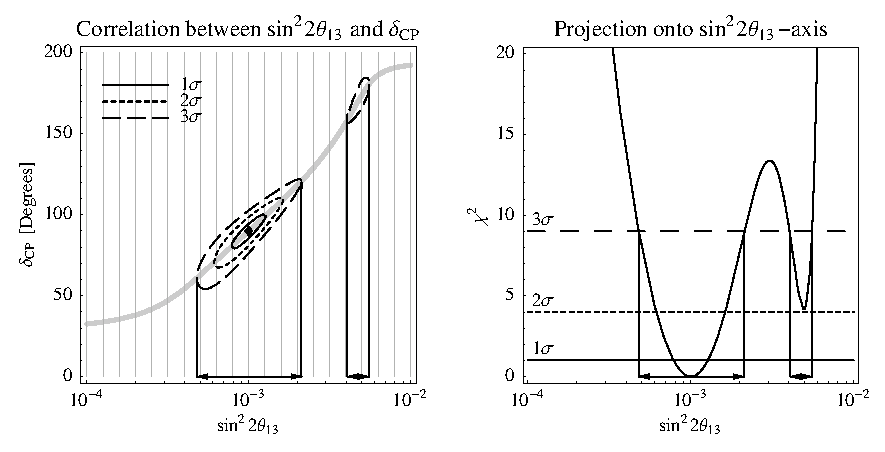
\includegraphics[width=16cm]{projex}
\end{center}
\mycaption{\label{fig:projex} Left plot: The correlation between $\stheta$ and $\deltacp$ as calculated in the example on page~\pageref{ex:corrth13dcp}, but for 1 d.o.f. only. Right plot: The $\chi^2$-value of the projection onto the $\stheta$-axis as function of $\stheta$. The projection onto the  $\stheta$-axis is obtained by finding the minimum $\chi^2$-value for each fixed value of $\stheta$ in the left-hand plot, \ie, along the gray vertical lines. The thick gray curve marks the position of these minima in the left-hand plot. The arrows mark the obtained fit ranges for $\stheta$ at the $3 \sigma$ confidence level (1 d.o.f.), \ie , the precision of $\stheta$.}
\end{figure}

\example{Projection of two- and $n$-dimensional manifold onto $\stheta$-axis}{
\label{ex:corrproj}

This example demonstrates how to use  {\tt ChiTheta} to project the fit manifold onto the $\stheta$-axis, \ie, how one can include correlations. We compute two sets of data: one for keeping all parameters but $\deltacp$ fixed (two-parameter correlations), and one for keeping all parameters free (multi-parameter correlation), but some external input for the solar parameters and $\rho$. Note that fixing all parameters but $\deltacp$ corresponds to imposing external knowledge on these parameters.

\begin{quote}
{\tt {\footnotesize
/\% Experiment initialization, set reference rate vector: \%/ \\
\mbox{ClearExp(); InitExperiment("{\tt NuFact2.exp}"); SetRunningTime(0,4.0); }\\
th12=arcsin(sqrt(0.8))/2; sdm=7e-5; th23=3.14/4; ldm=2e-3; \\
th13=arcsin(sqrt(0.001))/2; dcp=3.14/2; \\
\mbox{SetVacuumParameters(\{th12, th13, th23, dcp, sdm, ldm\}); SetRates();}\\
\\
/\%  Compute chi-square list with all but dcp fixed: \%/ \\
SetStartingValues(\{th12, th13, th23, dcp, sdm, ldm, 1.0\}); \\
\mbox{SetInputErrors(\{th12*0.001, 10, th23*0.001, 10, sdm*0.001, ldm*0.001, 0.001\});} \\
for (float x=-4; x<-2; x=x+2/20) \\
\mbox{\hspace*{0.5cm} Print(\{x,ChiDelta(x,\{th12, th13, th23, dcp, sdm, ldm, 1.0\}) \}); }\\
\\
/\% Compute chi-square list with all parameters free: \%/ \\
\mbox{/\% (but: 10\% prec. for solar params, 5\% for matter density) \%/} \\
SetStartingValues(\{th12, th13, th23, dcp, sdm, ldm, 1.0\}); \\
SetInputErrors(\{th12*0.1, 10, 10, 10, sdm*0.1, ldm, 0.05\}); \\
for (float x=-4; x<-2; x=x+2/20) \\
\mbox{\hspace*{0.5cm} Print(\{x,ChiDelta(x,\{th12, th13, th23, dcp, sdm, ldm, 1.0\}) \});}
}}
\end{quote}
The two lists of data then represent the $\stheta$ precisions with two-parameter correlations (gray-shaded) and multi-parameter correlations (arrows):
\begin{center}
\colorbox{white}{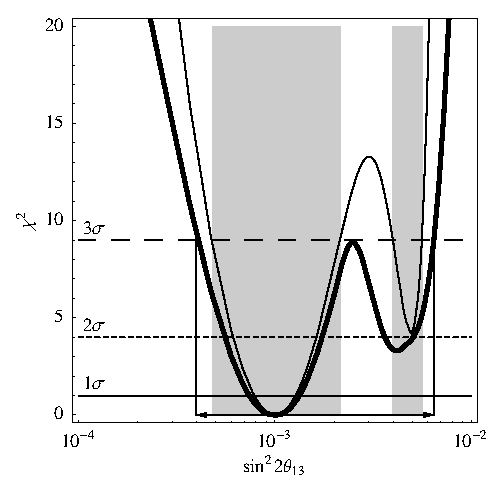
\includegraphics[width=6cm]{projallex}}

\vspace*{0.1cm}

\footnotesize{(Same parameters as on page~\pageref{ex:corrth13dcp} and in \figu{projex}, but 1 d.o.f.)}
\end{center}
}

\section{The treatment of external input}

\bi
\item
 Treatment of external input: short introduction to priors
\item
 The effect of the starting values and input errors
\item
 Functions SetStartingValues, SetInputErrors to be called first
\item
 What for negative hierarchy? Defintion of $-\ldm - \sdm$?
\ei

\section[Projection onto the $\theta_{13}$-axis or $\deltacp$-axis]{Projection onto the $\boldsymbol{\theta_{13}}$- or $\boldsymbol{\deltacp}$-axis}

\bi
\item
 Call SetStartingValues and InputErrors first \ra\ three sets of parameters 
\item
 Single and multiple experiments: ChiDelta and ChiTheta + single funtions \ra\ return values;
mention that $\chi^2$ does not add anymore; general parameter transfer concept
\item
 The effect of the starting point of the minimizer
\item
 What these functions do \ra\ figure
\item
 Refer to example: code
\item
 When does it not work: jumps \ra\ modify starting point accordingly
\ei

\section[Projection onto any hyperplane]{Projection onto any  hyperplane}

General form and especially: DeltaTheta-Minimizer; mention calculation time!

\chapter{Finding degenerate solutions}

\bi
\item
 Single- and multiple experiment support
\item 
Example: Finding degenerate solutions with multiple experiments!?
\item
 What does that do?
\item
 Example: how to treat sign-degeneracy in th13-limit
\ei

\chapter{Obtaining low-level information}

\bi
\item
 Obtaining rate vectors
\item
 Obtaining fluxes/cross sections etc.
\item
 ``Check''-functions
\ei

\chapter{Changing experiment parameters at running time}

\bi
\item
 Baseline, Target mass, Source power, running time
\item
 Matter density profile
\item
 Threshold function, efficiencies etc.
\ei